\addchap{\lsPrefaceTitle}
 
A few words first about the origin of my own interest in the history
of our field. My undergraduate education in Linguistics came
simultaneously from two strong representatives of the American
Structuralist tradition, \name{William M.}{Austin} and \name{Alva L.}{Davis}, and from
one of the very first graduates of the program at MIT to teach in
another major institution, \name{James D.}{McCawley}. The manifest
incompatibilities between these two world views made me wonder just
where the field had come from, and the course offered at the 1966
{Linguistic Institute} by Sir \name{John}{Lyons} initiated me into a sense of
how rich and complex that background was. When I entered the MIT
program the following fall, my initial intention was to produce a
dissertation on the history of linguistics. Although that didn't come
to pass, my interest in such a study did not go away, and was in fact
reinforced by discussions with colleagues and faculty, and especially
by \name{Paul}{Kiparsky}'s fine classes in what was misleadingly referred to
by MIT students of the time as ``the Bad Guys course''.

When I had the opportunity to spend a wonderful sabbatical year in
Copenhagen in 1972--73 with the support of a Fellowship from the ACLS,
I was privileged to benefit from the cordial hospitality and
assistance of \name{Eli}{Fischer-Jørgen\-sen} (section~\ref{sec:eli}
below). Eli also had me read and comment on the developing
manu\-script of her own magisterial survey of the history of phonology
\citep{fischer-jorgensen75:trends}, and encouraged me in the idea of
doing something similar from a different perspective. That possibility
came closer to fruition when \name{Vicki}{Fromkin} turned her history of
linguistics course at UCLA over to me in 1981, and another ACLS
Fellowship allowed me to undertake the first edition of this book
during my stay in Geneva starting the following year, as described in
the preface to the first edition below.

The reception of that work was in general (though not universally)
gratifyingly positive, an impression reinforced by the fact that
translations have appeared in \ili{Spanish} (by Elena and Miguel Aparicio,
published as \textsl{La fonologia en el siglo XX} by Editiones Antonio
Machado, 1990) and most recently, in \ili{Chinese} (as 二十世纪音系学,
translated
by Changliang Qu with a new preface, published by The Commercial
Press, Beijing, 2016).

It did not take long, however, for it to become obvious that
publishing a book entitled \textsl{Phonology in the Twentieth Century}
in 1985 was remarkably foolish. In fact the late 1980s and early 1990s
were a time of special turbulence in phonological theory, and by the
end of the century things looked quite different than they had when I
wrote in the early 1980s. A number of developments, some discussed in
chapters~\ref{ch.spe} and~\ref{ch.otlabphon} below, marked the
dissolution of the consensus loosely characterizable as that of
``post-\textsl{SPE}'' phonology, and the appearance of
\citealt{prince:smolensky:optimality} brought a radically new set of
problems and perspectives, not foreseen in the original edition of
this work, to prominence, as described below in
chapter~\ref{ch.otlabphon}. I also note there the emergence of a
distinct line of theorizing about the nature of phonology, the 
\isi{Laboratory Phonology} movement, which has sought to return the study of
\isi{sound structure} to its phonetic roots.

In addition, new scholarship has appeared on many of the topics and
central figures of the book as originally conceived, and it is
appropriate to incorporate as much of that work as
possible. Accordingly, the aim of the present edition is in part to
update the accounts previously offered of phonologists and their
research, and to extend the picture presented in a way that brings us
more authentically to the turn of the century, while also fleshing out
the references and noting relevant work that has appeared since the
first edition.

I am appreciative of the suggestions and corrections in the reviews
that have appeared, especially the reviews by \name{Kenneth}{Howell}
(\textsl{Historiographica Linguistica} XIII: 85--91, 1986), \name{Roger}{Lass}
(\textsl{Journal of Linguistics} 23:476-481, 1987) and 
\name{Eli}{Fischer-Jørgensen} (\textsl{Phonetica} 44:192-195, 1987). I am
especially grateful to the late \name{Stephen O.}{Murray} for his remarks in a
survey article (\textsl{Historiographica Linguistica} XVI:149--171,
1989) and for a set of detailed comments on the text which he provided
me. I am sad that I will not be able to discuss the revised book with
him.

I would also like to thank \name{Elan}{Dresher} and \name{Harry}{van der Hulst} for sharing
with me chapters of their forthcoming Oxford University Press volume
the \textsl{Oxford Handbook of the History of Phonology}.  The diverse
perspectives presented there on the topics of the present work (among
others) form a very useful complement to my own presentation, and I
have learned a lot (some of which is incorporated here) from reading
this material, which has also highlighted items in the literature that
are relevant to my account.

In addition to minor editorial changes and enlarging both the coverage
and the references beyond their original form, I have tried to correct
errors of fact and interpretation. Where other views have been
developed in the literature, but where I feel that my original
analysis is reasonable, I have let that stand in substance rather than
trying to engage with all alternative interpretations of the
history. I am sure those with differing perspectives will feel free to
expand on our differences.

In addition to those listed above, I am extremely grateful for
comments and suggestions offered by students and faculty colleagues at
UCLA, Stanford, Johns Hopkins and Yale in courses covering this
material. I have attempted to incorporate as many as possible of these
varied observations in this revision. Needless to say, the errors and
misunderstandings that remain are entirely mine.

I am pleased to acknowledge the generosity of the University of
Chicago Press, publishers of the first edition of this work, in
reverting the rights to the book to me so that the present revised
edition could be published by Language Science Press. In the course of preparing it, Sebastian Nordhoff and Felix Kopecky have provided invaluable help with LaTeX and other production issues.

I am very grateful to those who helped me find relevant material,
including especially the photographs of scholars discussed in this
book which I hope will bring a bit more life to the text. Those to
whom I am indebted include \name{Hans}{Basbøll}, \name{Joan}{Bybee}, \name{Patricia}{Donegan},
\name{Andrew}{Garrett}, \name{Frans}{Gregersen}, John\ia{Halle, John} and \name{Tim}{Halle}, \name{Larry}{Horn}, \name{John}{Joseph}, \name{Paul}{Kiparsky}, \name{Bob}{Ladd}, \name{Fritz}{Newmeyer}, \name{Joe}{Salmons}, \name{David}{Sapir}, Jacques\ia{de Saussure, Jacques} and \name{Louis}{de Saussure}, \name{Gunver}{Skytte}, \name{William}{Twaddell}
and \name{Bert}{Vaux}. Action shots of the founding of modern linguistics
appear
courtesy of Halle family.\\[3ex]



\begin{center}
  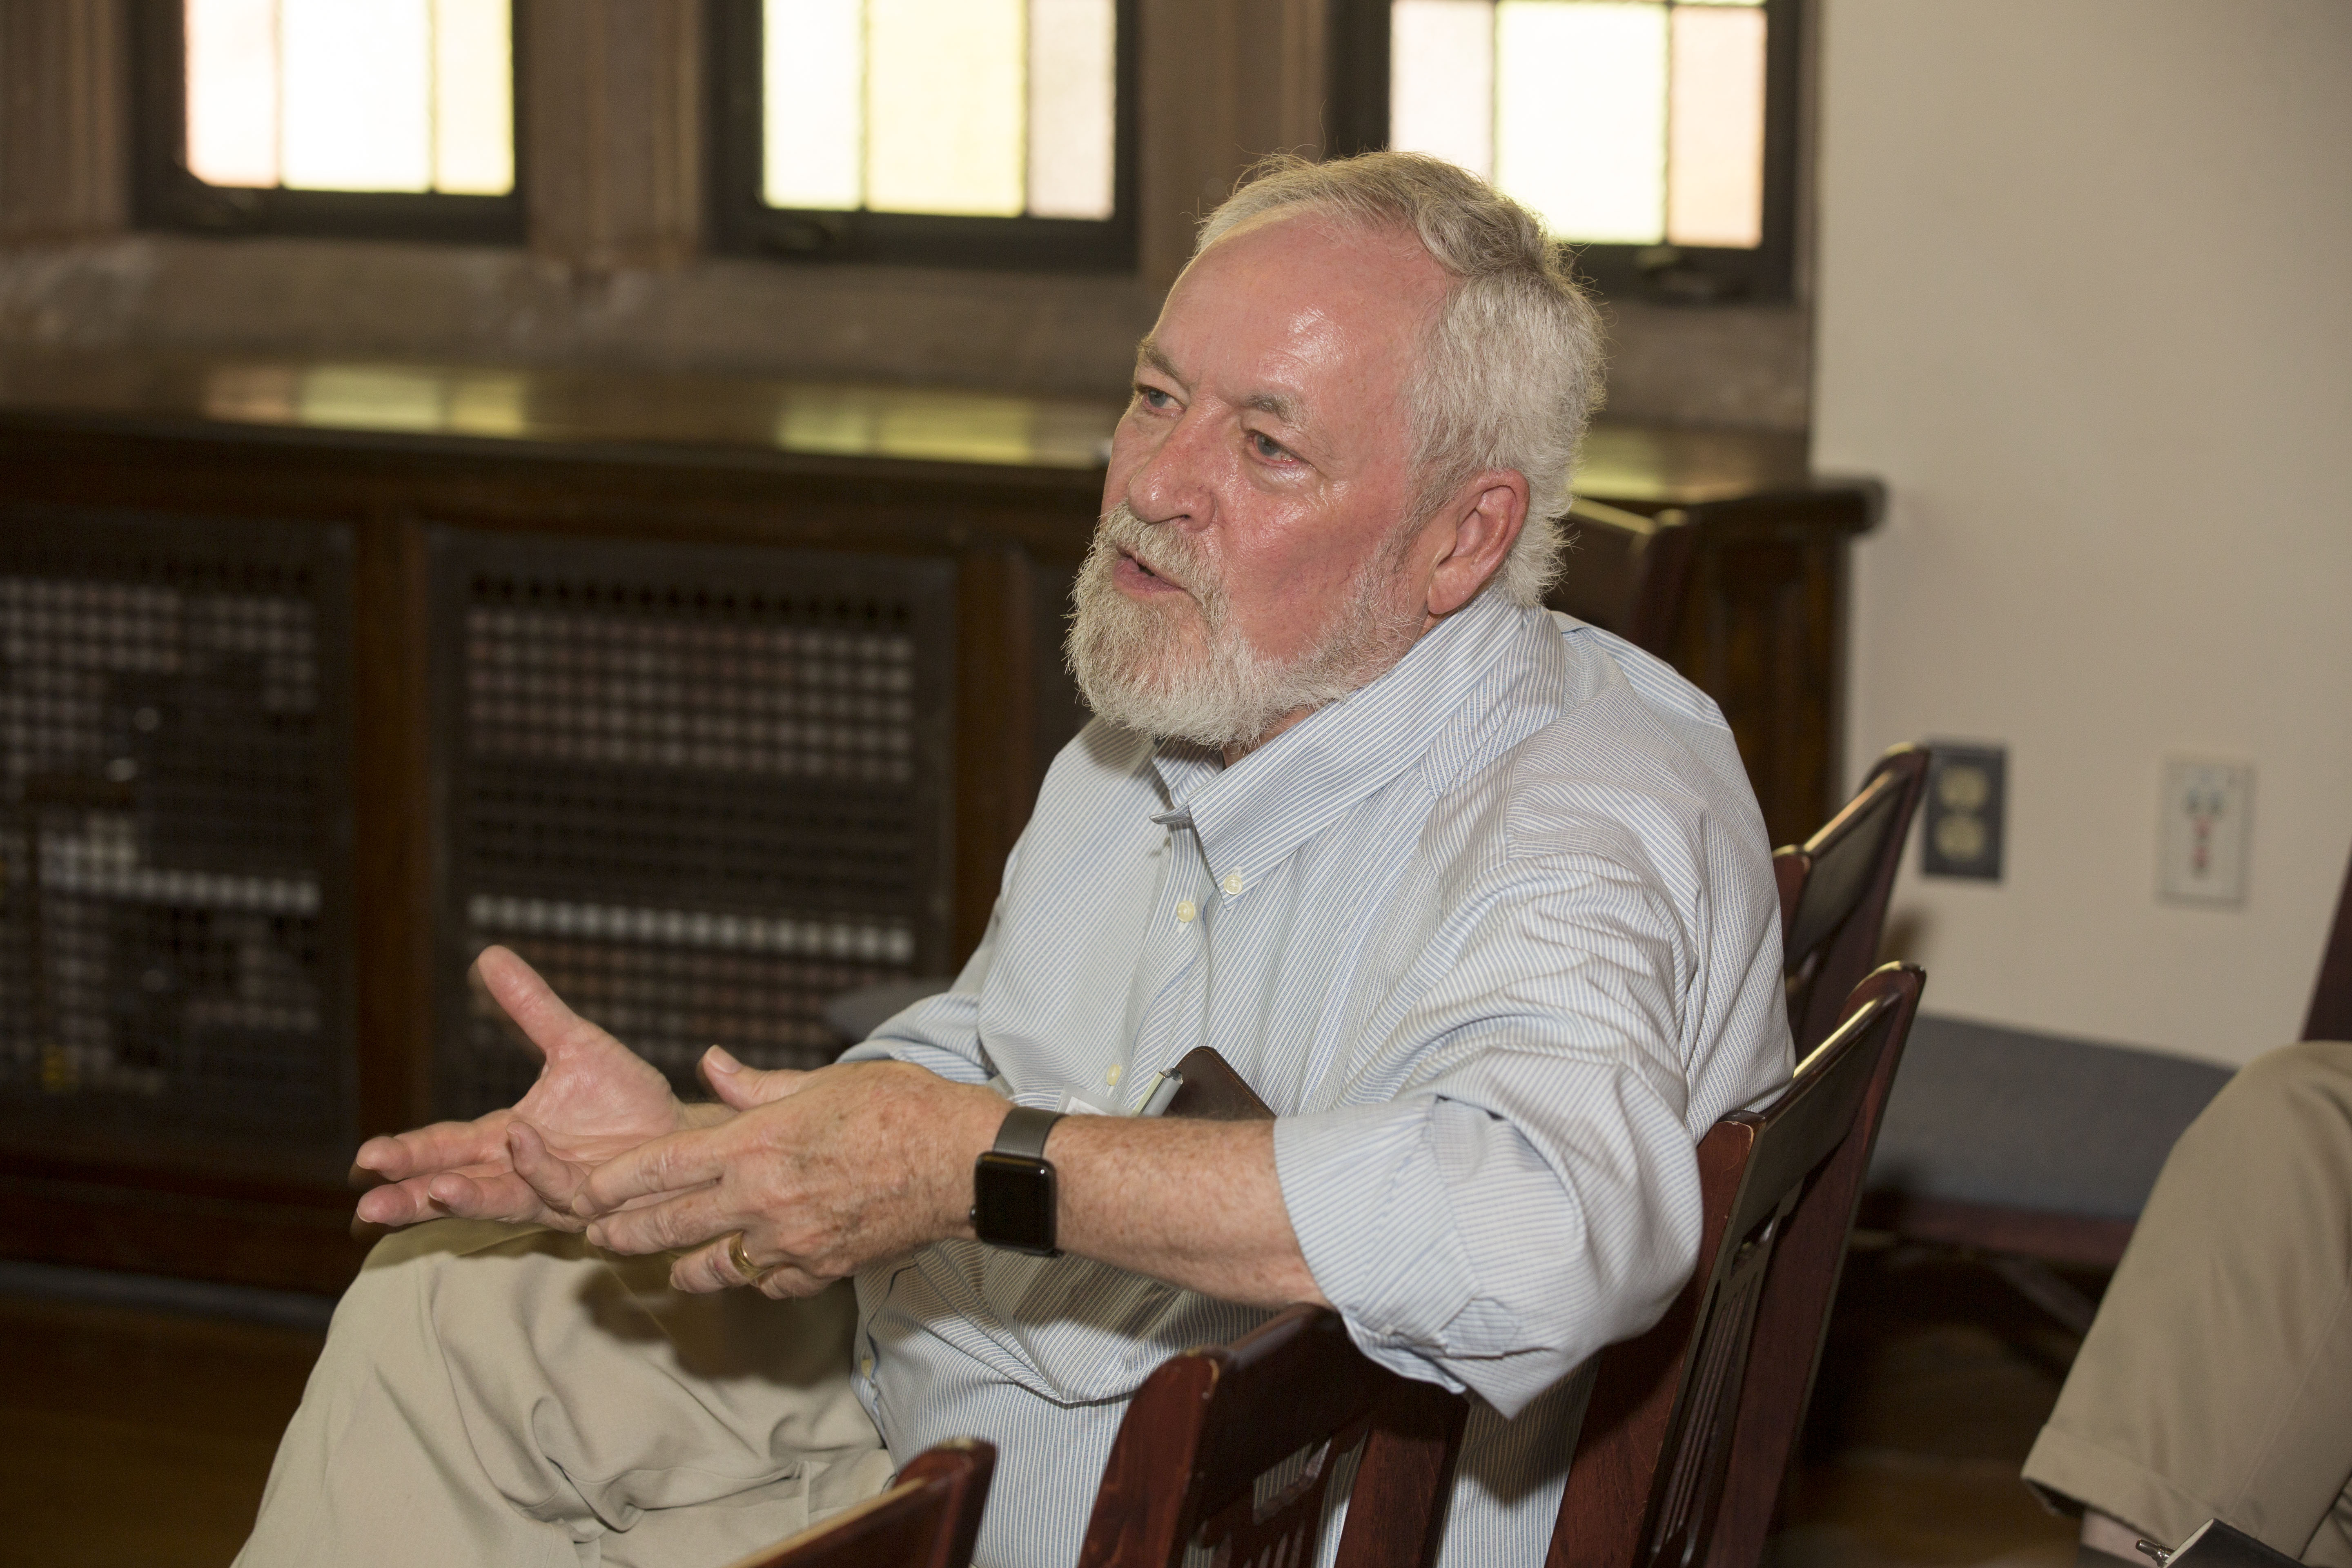
\includegraphics[width=.5\textwidth]{figures/sra_symposium.jpg}\\
  \name{Stephen R.}{Anderson}\\(Photo by Harold Shapiro)
\end{center}

%%% Local Variables: 
%%% mode: latex
%%% TeX-master: "/Users/sra/Dropbox/Docs/Books/P20C_2/LSP/main.tex"
%%% End: 
